\chapter{User Interface Design \\
\small{\textit{-- Ryan Davis, Roy Tas, and Cory Vitanza}}
\index{user interface design} 
\index{Chapter!UserInterfaceDesign}
\label{Chapter::UserInterfaceDesign}}

% ======================================================
% USER PERSONAS
% ======================================================
\section{User Persona}

% --------------------------- Maria Davis ---------------------------
\subsection*{Maria Davis}
\begin{itemize}[leftmargin=2em]
    \item \textbf{Age:} 42 years old
    \item \textbf{Family Status:} Full-time caregiver for her 80-year-old mother (early dementia)
    \item \textbf{Location:} Brooklyn, NY
    \item \textbf{Occupation:} Part-time dental assistant
    \item \textbf{Background:} Moved her mother in last year after wandering incidents
    \item \textbf{Core Challenge:} Balancing work, kids, and caregiving; high morning anxiety
    \item \textbf{Required Solution Features:}
        \begin{itemize}
            \item Simple and dependable device
            \item Immediate geo-fence notifications
            \item Reduced need for continuous supervision
        \end{itemize}
\end{itemize}

% --------------------------- John Smith ---------------------------
\subsection*{John Smith}
\begin{itemize}[leftmargin=2em]
    \item \textbf{Age:} 10 years old
    \item \textbf{Condition:} Diagnosed with autism
    \item \textbf{Location:} Paramus, NJ
    \item \textbf{Wandering Triggers:} Stressful or crowded environments (malls, airports)
    \item \textbf{Personality:} Smart, curious, active; enjoys technology
    \item \textbf{Device Preferences:}
        \begin{itemize}
            \item Prefers small wearable devices
            \item Dislikes bulky devices
        \end{itemize}
    \item \textbf{Required Solution Features:}
        \begin{itemize}
            \item Real-time location updates for parents
            \item Quick distance + geo-fence alerts
            \item Simple UI for school staff
        \end{itemize}
\end{itemize}

% --------------------------- Brian Cleary ---------------------------
\subsection*{Brian Cleary}
\begin{itemize}[leftmargin=2em]
    \item \textbf{Age:} 67 years old
    \item \textbf{Status:} Retired mechanic living alone
    \item \textbf{Location:} Weehawken, NJ
    \item \textbf{Health Concerns:} Dizziness; fall risk; forgets to charge devices
    \item \textbf{Routine:} Morning walks by the Hudson River
    \item \textbf{Device Preferences:}
        \begin{itemize}
            \item Prefers extremely simple or automatic devices
            \item Avoids smartphones
        \end{itemize}
    \item \textbf{Required Solution Features:}
        \begin{itemize}
            \item Long battery life
            \item Automatic fall detection
            \item Passive well-being updates for family
        \end{itemize}
\end{itemize}

\section{User Interface Design}

Figma Paper Prototype:  
\url{https://www.figma.com/make/jALgOM7hNgKhoa1sMRlw5L/User-Interface-for-Tracking-App?node-id=0-4}

% ------------ Figure 1 --------------------
\begin{figure}[!htbp]
    \centering
    \vspace{1em}
    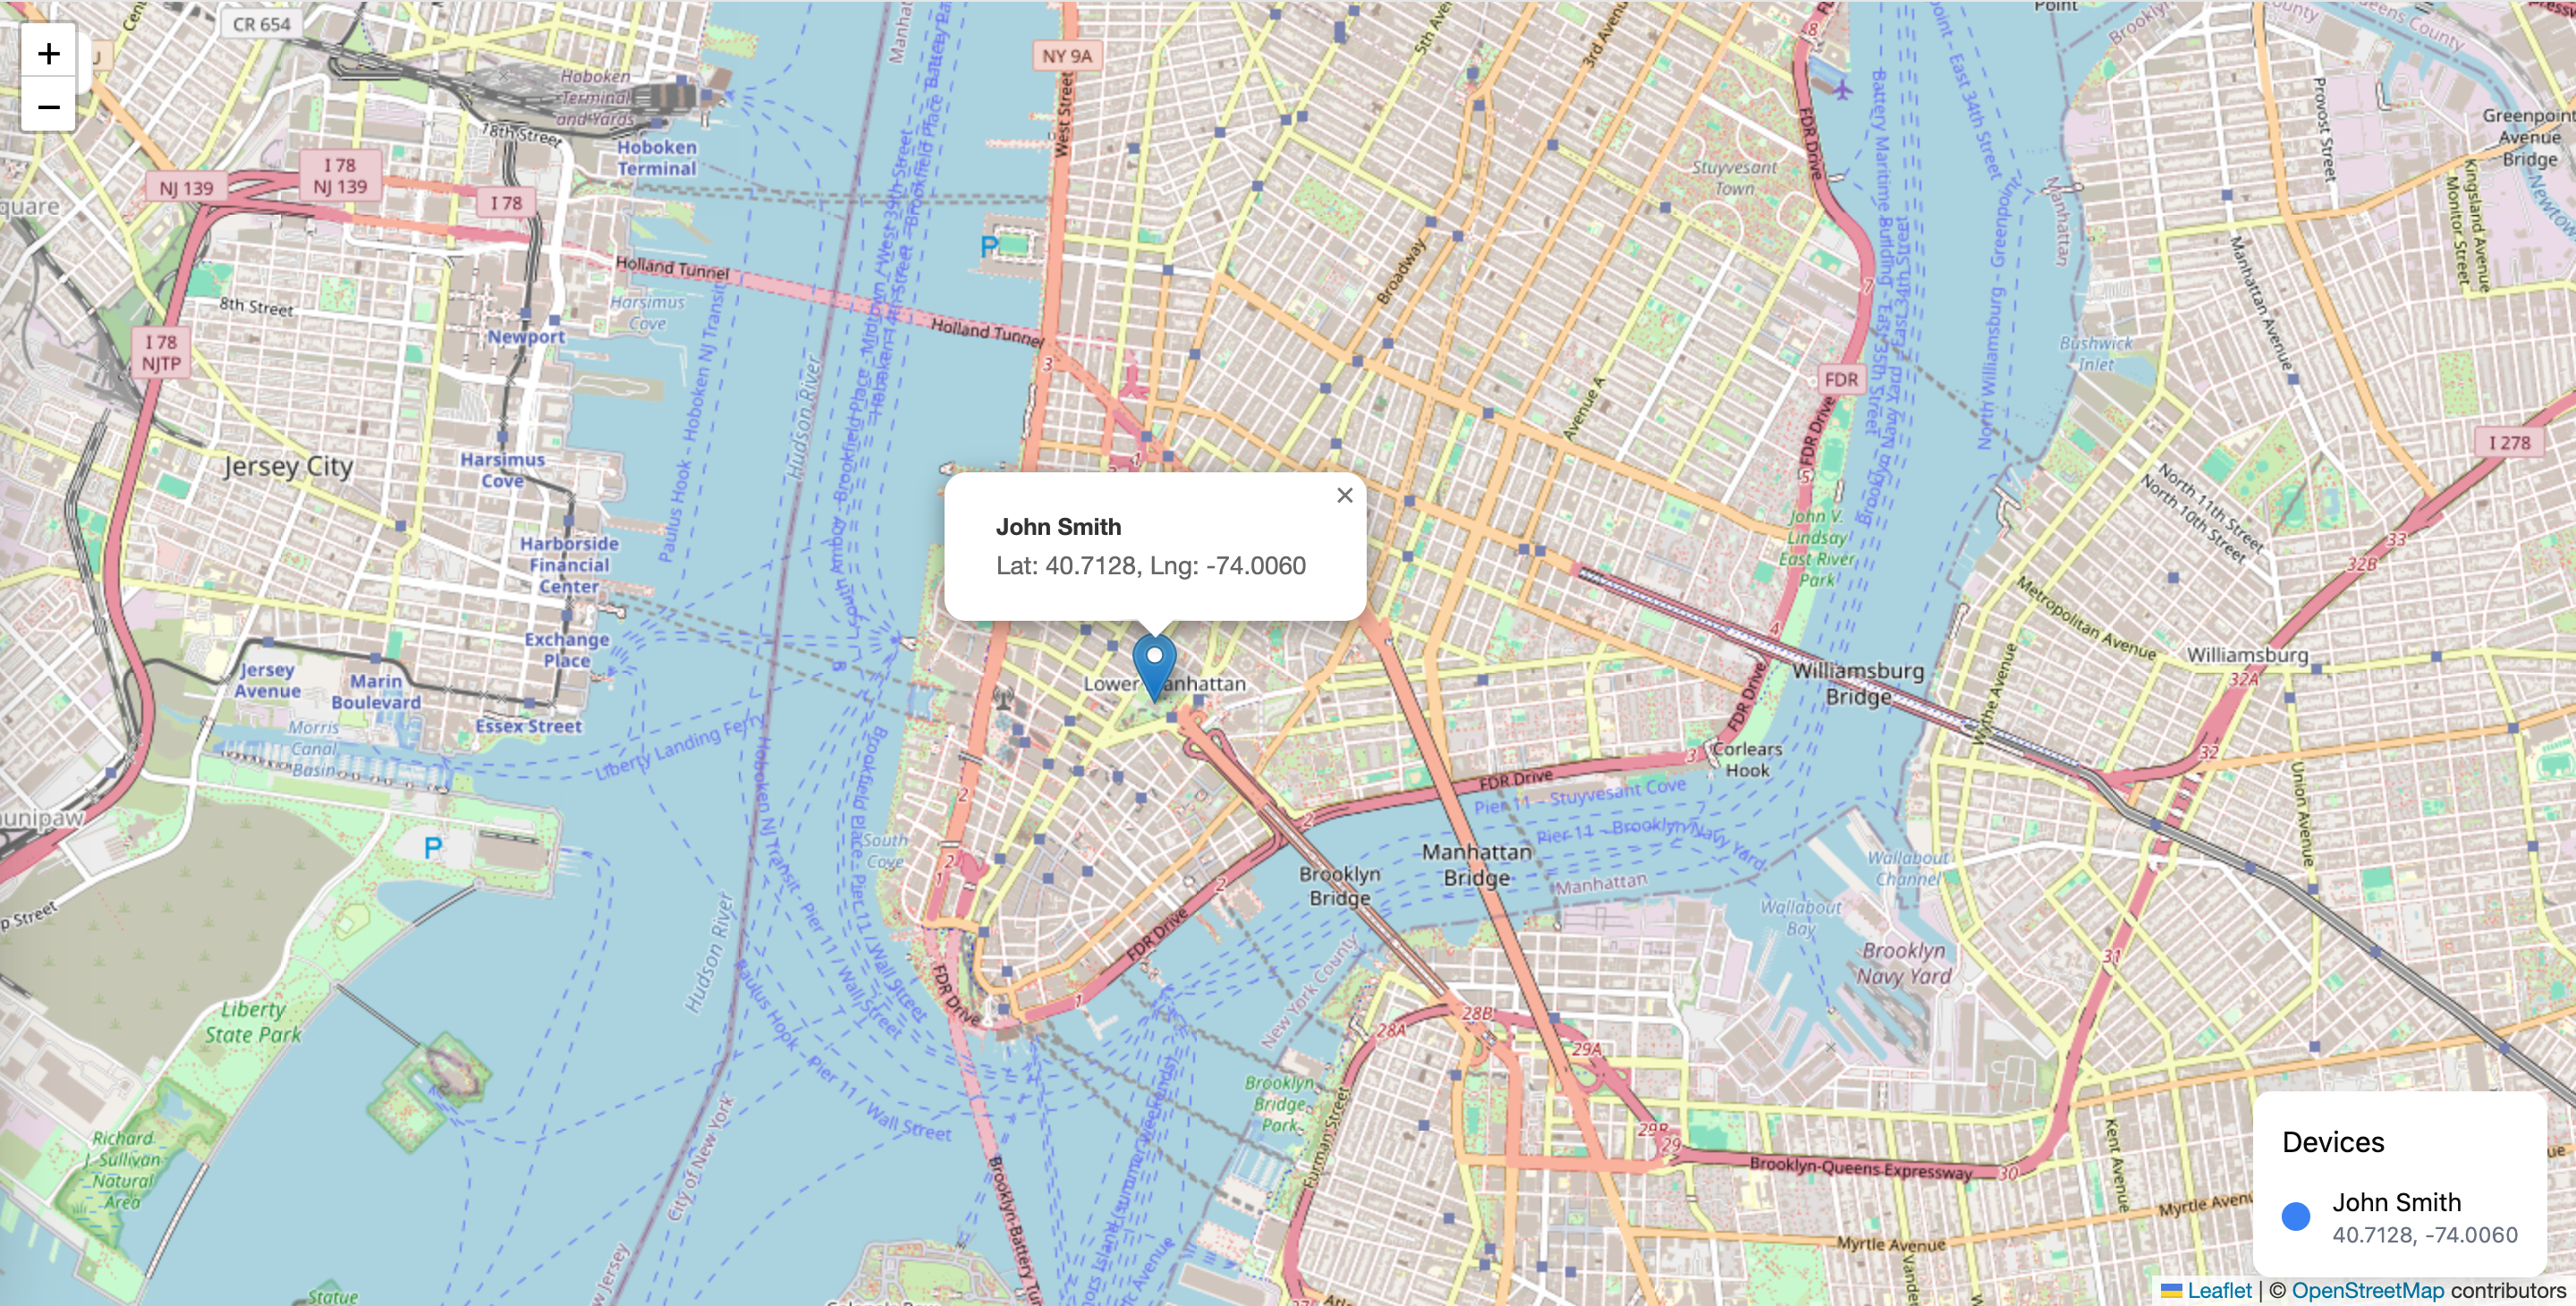
\includegraphics[width=0.75\textwidth]{png/screenshots/FigmaUISS.png}
    \caption{\FigureLabel{PaperPrototype}: Figma Paper Prototype for FindIt UI.}
    \label{fig:figmaUI}
    \vspace{1em}
\end{figure}

% ------------ Figure 2 --------------------
\begin{figure}[!htbp]
    \centering
    \vspace{1em}
    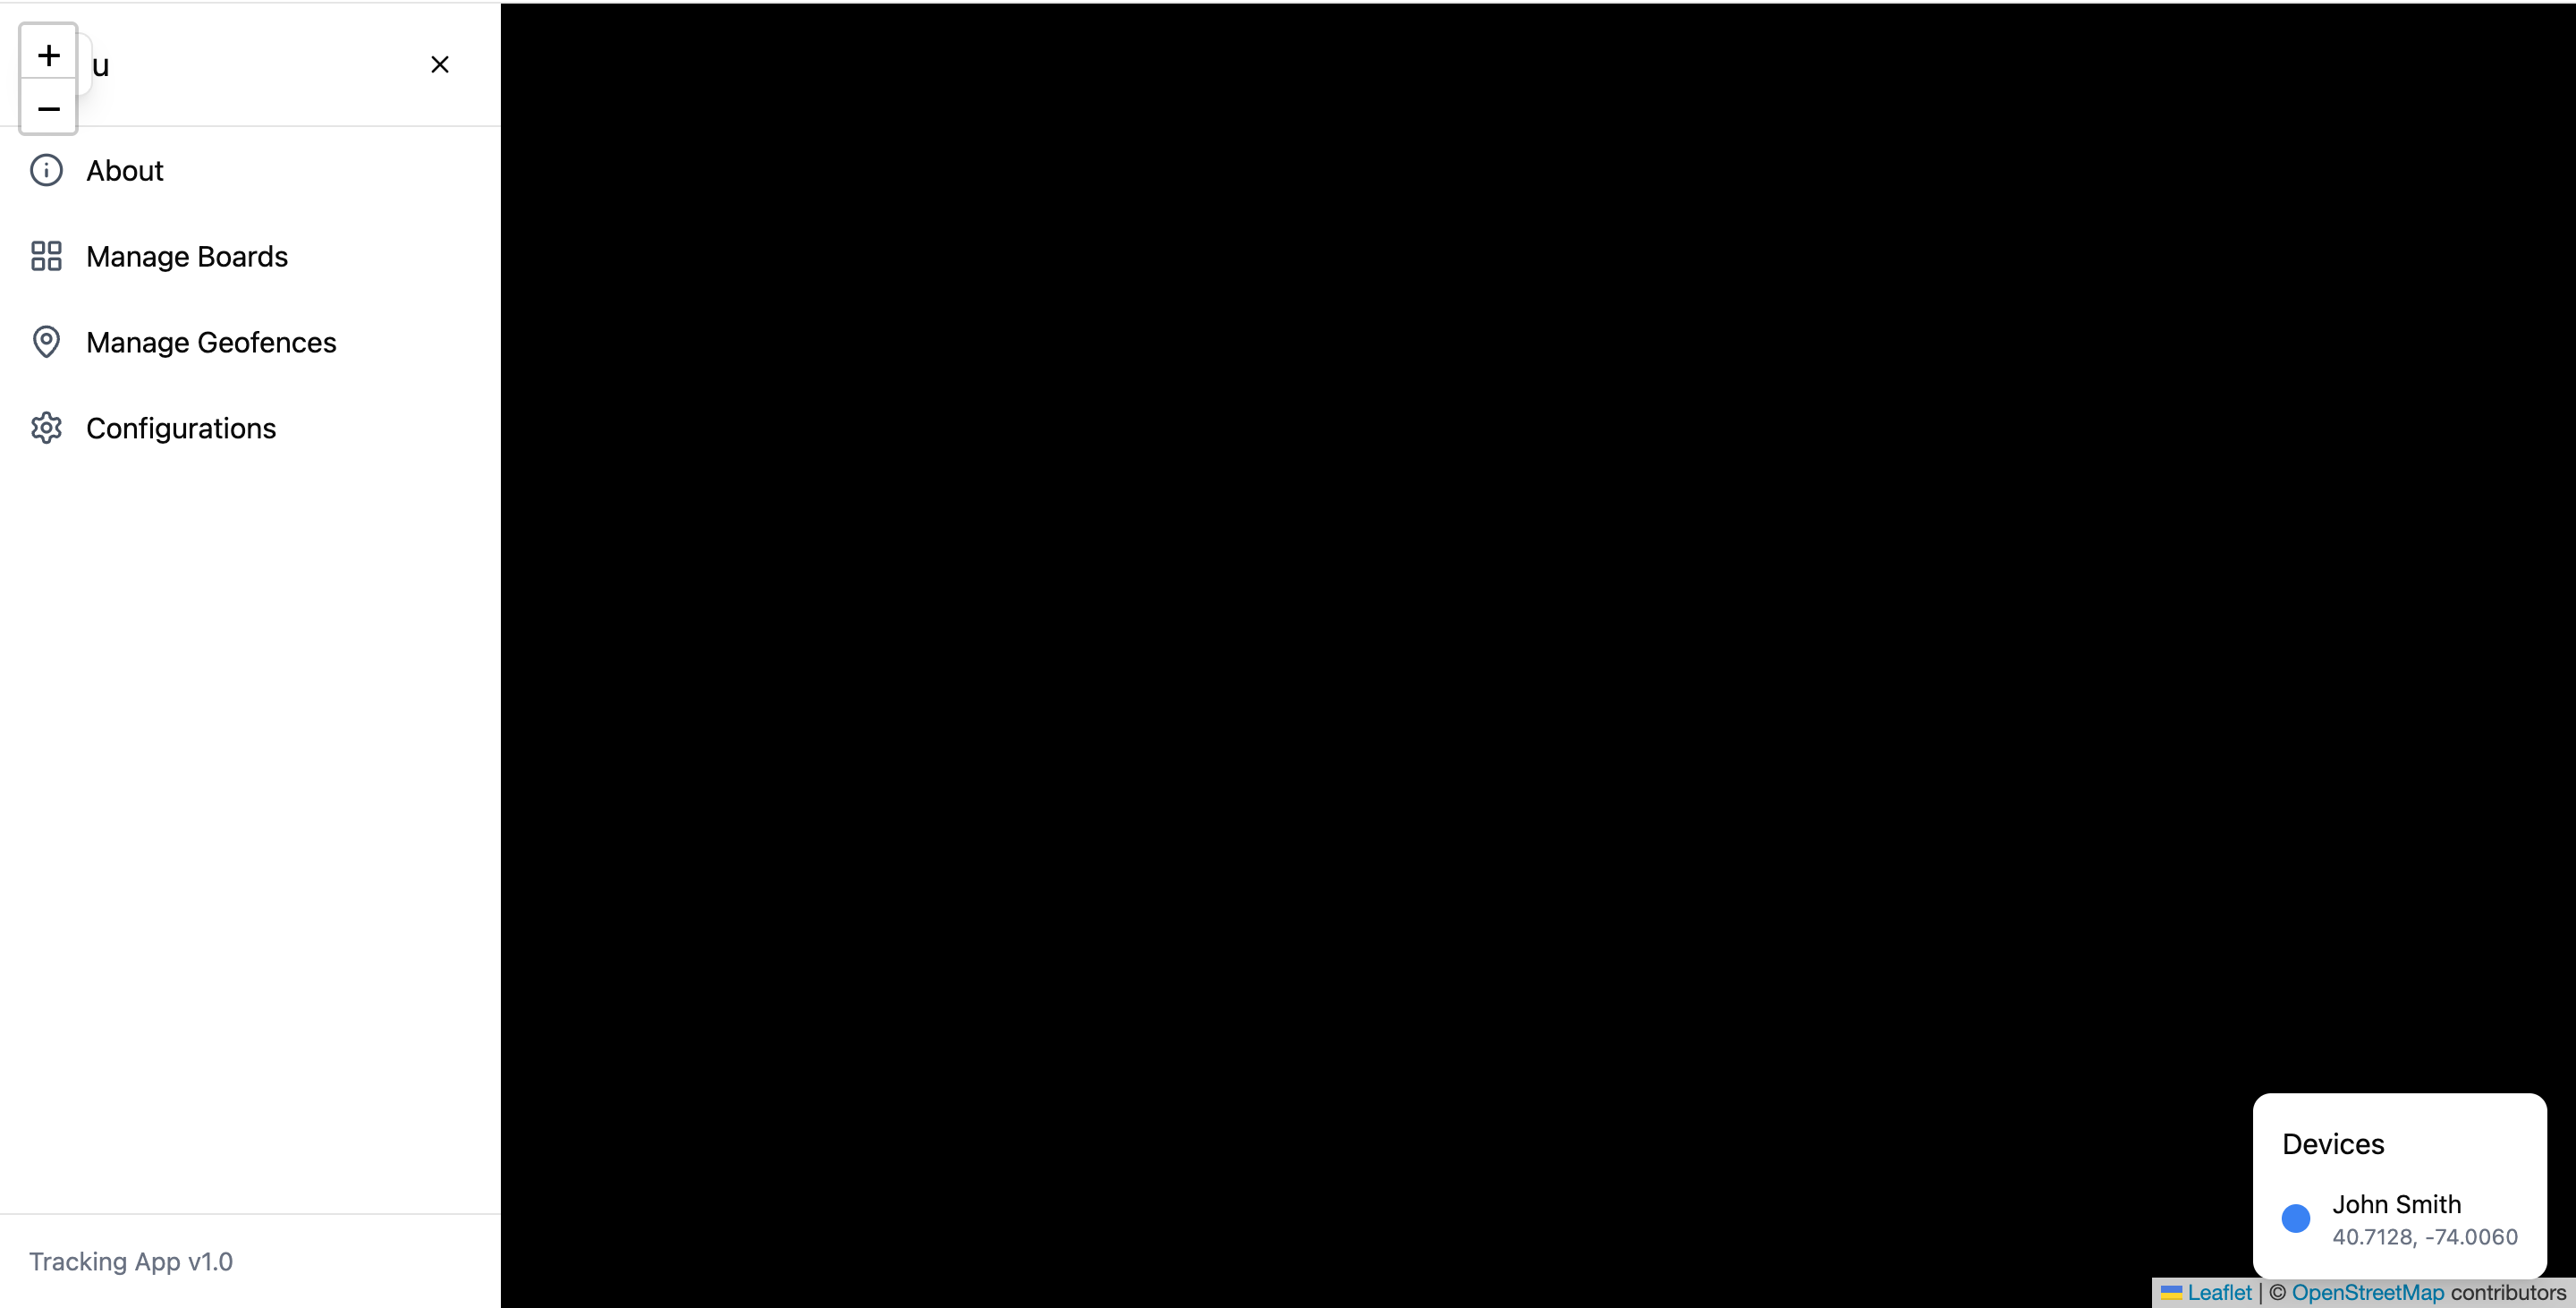
\includegraphics[width=0.75\textwidth]{png/screenshots/UISideMenu.png}
    \caption{\FigureLabel{PaperPrototype}: Figma Paper Prototype of Side Menu.}
    \label{fig:FigmaMenu}
    \vspace{1em}
\end{figure}

% ------------ Figure 3 --------------------
\begin{figure}[!htbp]
    \centering
    \vspace{1em}
    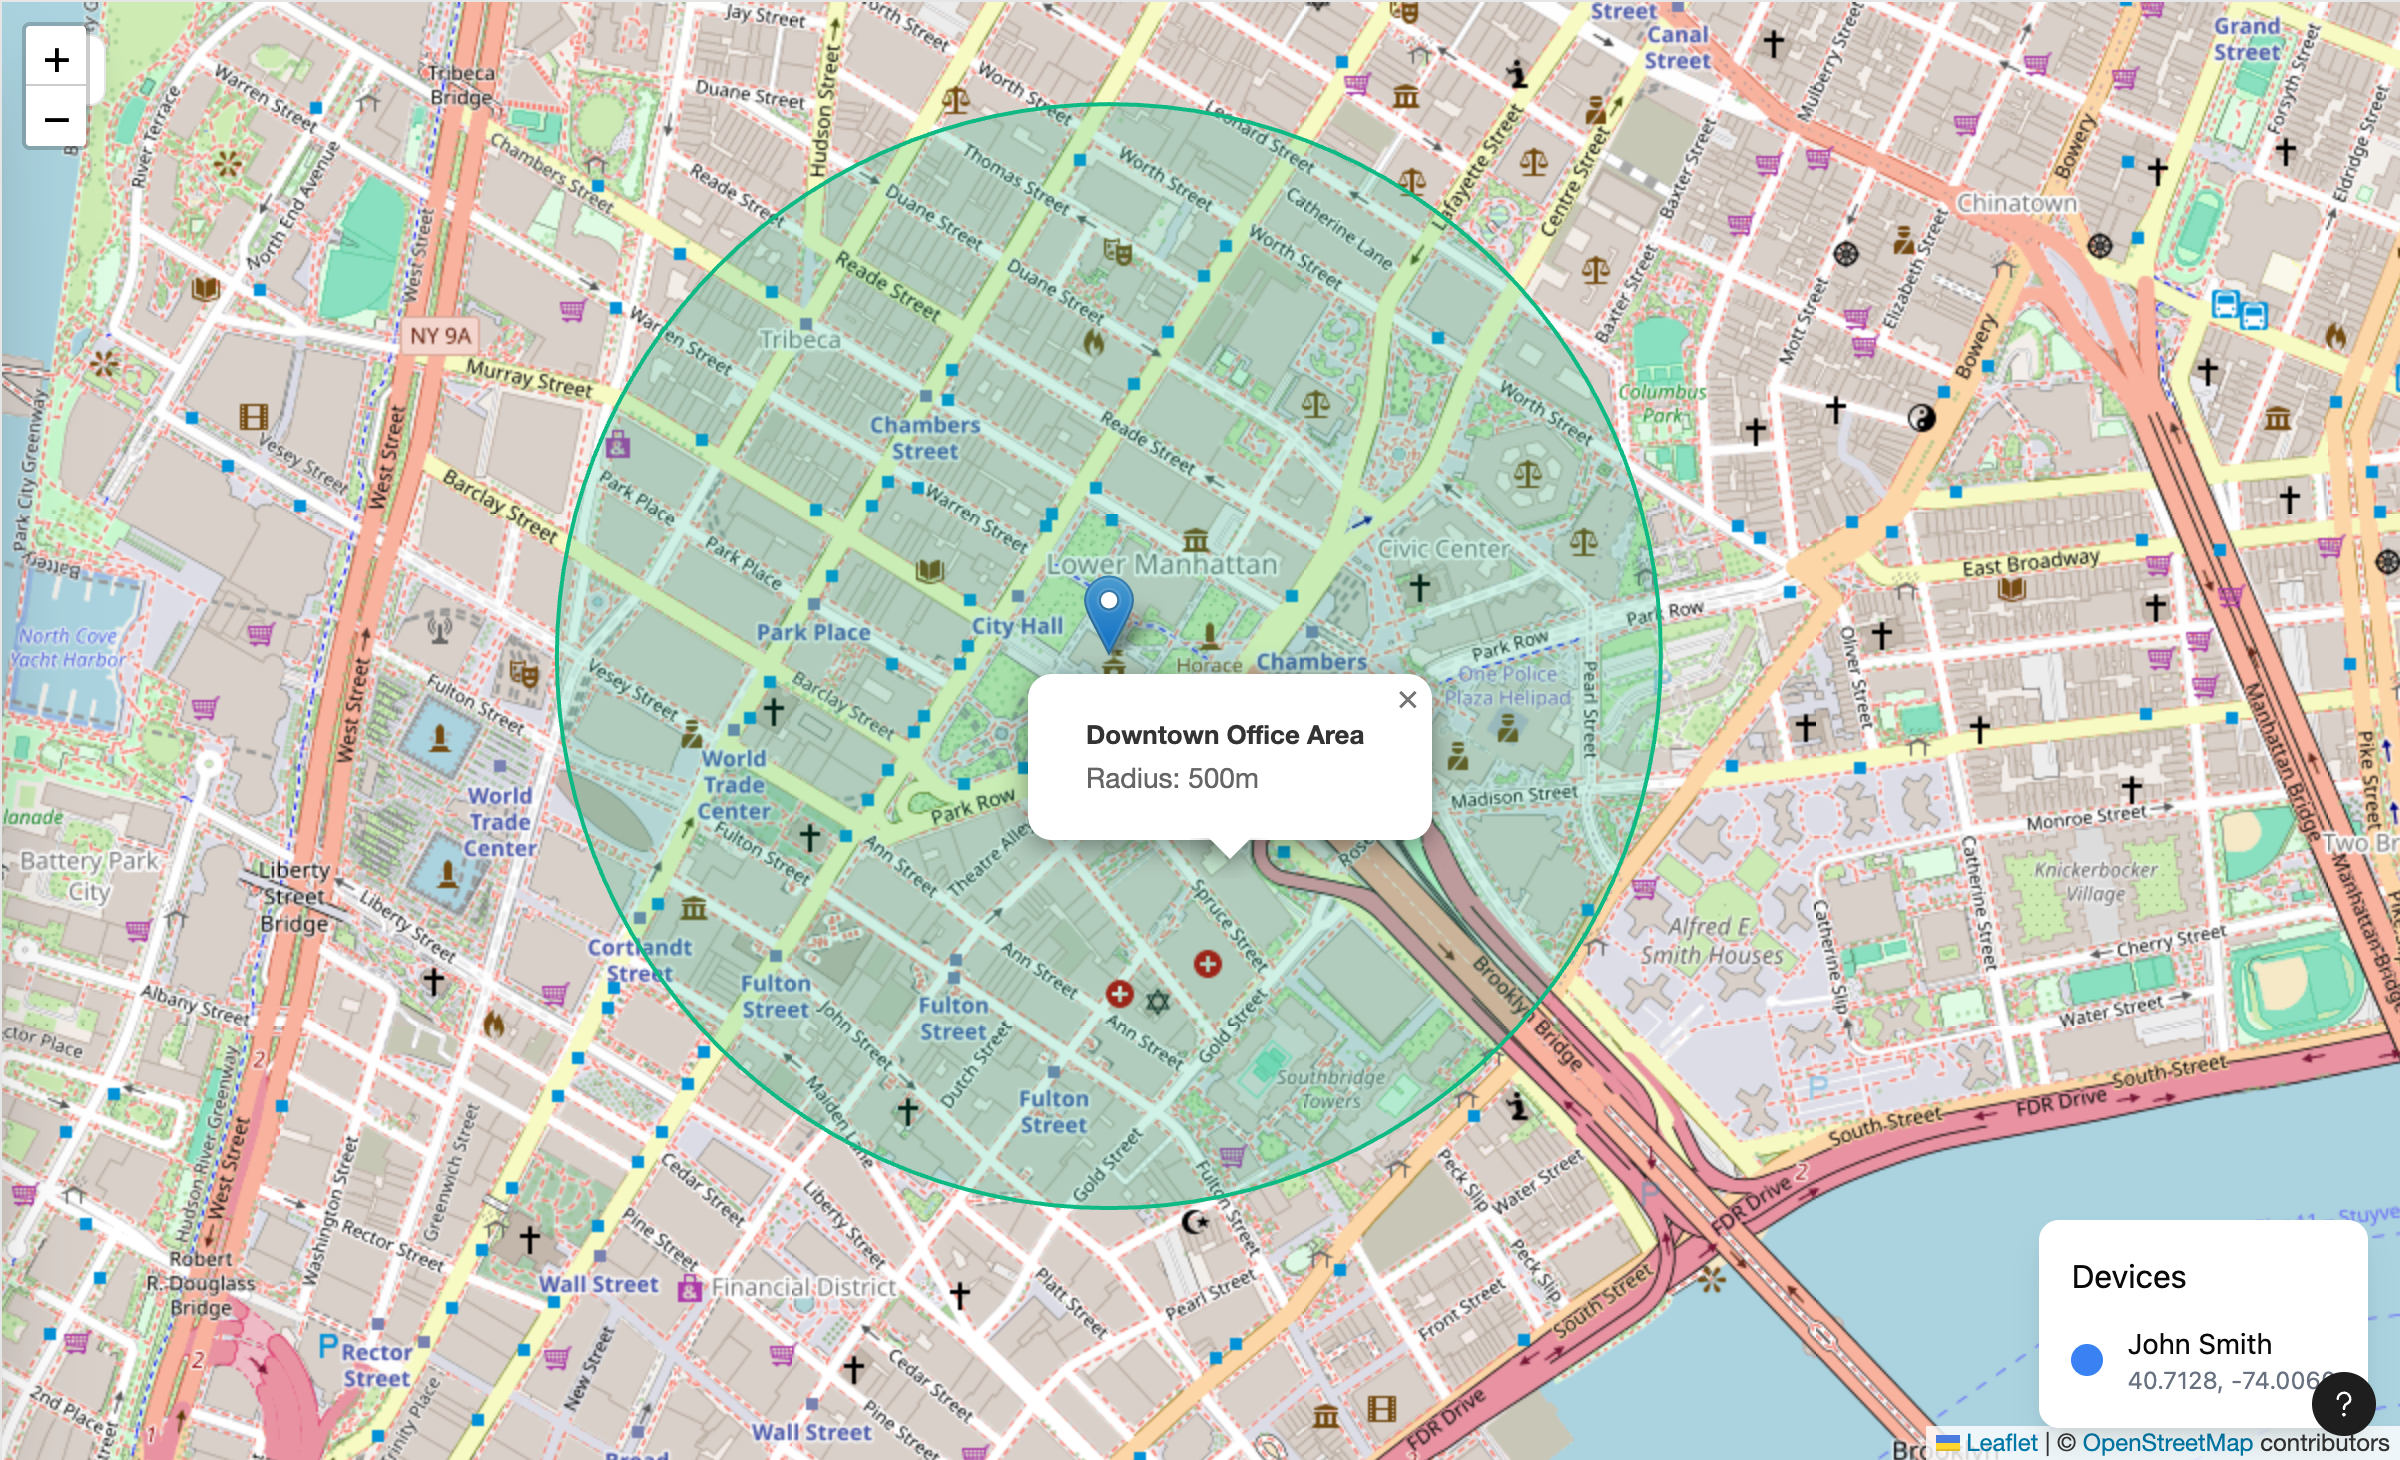
\includegraphics[width=0.75\textwidth]{png/screenshots/geofenceFigma.png}
    \caption{\FigureLabel{PaperPrototype}: Figma Paper Prototype of Geofence Implementation.}
    \label{fig:FigmaGeofence}
    \vspace{1em}
\end{figure}
